\chapter{Campo Gravitomagnético ***PRELIMINAR***}\label{cap:gravito}

\section{Introducción}

En RG toda forma de energía \textit{y momentum} contribuye a modificar la geometría del espaciotiempo a su alrededor y con ello a producir lo que llamamos campo gravitacional. Así, por ejemplo, el Sol al estar rotando, produce un campo gravitacional diferente en el sistema solar, comparado con el caso en que éste estuviese estático. Esto representa una gran diferencia respecto a la teoría de Newton de la Gravitación, donde sólo la densidad de masa de los cuerpos es fuente de campo gravitacional y por lo tanto el campo gravitacional del Sol es independiente de su rotación.

Sin embargo, y como es de esperar, en regiones con campos gravitacionales débiles los efectos predichos por RG debido al movimiento de las fuentes son en general varios órdenes de magnitud menores que los causados por su densidad de masa (o densidad de energía).

En este capítulo se estudiarán, \textit{dentro de la aproximación de campo débil} (primer orden en la expansión en potencias de $G$), los efectos gravitacionales causados por el movimiento, y \textit{en especial por la rotación}, de las fuentes. Es interesante comprobar que la descripción resulta ser muy análoga a la de los campos eléctricos y magnéticos en electrodinámica clásica, pues ciertas componentes de la perturbación de la métrica a primer orden dependerán de la densidad y del flujo de masa de la fuente, de forma similar a la que los \textit{potenciales electromagnéticos} dependen de la densidad de carga y corriente. Debido a esto, el análogo gravitacional del campo magnético recibe en ocasiones el nombre de \textit{campo gravitomagnético} y es de especial interés puesto que, a diferencia del ``campo gravitoeléctrico'', no tiene contraparte en la teoría gravitacional newtoniana.


\section{Caso de una distribución de materia no-relativista sin presión}\label{sec:CDNR}

En este caso, podemos usar la expresión para el tensor de energía-momentum de
polvo. En el régimen no-relativista, donde las velocidades de las partículas
que constituyen el polvo son muy bajas comparadas con la velocidad de la luz,
tenemos que, a primer orden en $v^i/c$,
\begin{equation}\label{Tem0norel}
(T^{(0)})_{00}\approx \rho c^2, \qquad (T^{(0)})_{0i}\approx -\rho cv^i, \qquad (T^{(0)})_{ij}\approx 0,
\end{equation}
donde $\rho$ es la densidad (propia) de masa. De este modo (\ref{solh}) implica que
\begin{eqnarray}
\bar{h}_{00}(\vec{x},t)&\approx&-\frac{4G}{c^2}\int\frac{\rho(\vec{x}',t_{\rm ret})}{\left|\vec{x}-\vec{x}'\right|}\, d^3x' \\
&=&\frac{4}{c^2}\phi_{\rm ret}, \label{hbar00}
\end{eqnarray}
donde
\begin{equation}\label{defphii}
 \phi_{\rm ret}(\vec{x},t):=-G\int\frac{\rho(\vec{x}',t_{\rm ret})}{\left|\vec{x}-\vec{x}'\right|}\, d^3x'
\end{equation}
denota el potencial newtoniano \textit{retardado}, ya que $t_{\rm ret}=t-|\vec{x}-\vec{x}'|/c$. Además, 
\begin{eqnarray}
\bar{h}_{0i}(\vec{x},t)&\approx& \frac{4G}{c^3}\int\frac{(\rho v^i)(\vec{x}',t_{\rm ret})}{\left|\vec{x}-\vec{x}'\right|}\, d^3x' =-\frac{1}{c^2}A^i_{\rm ret}, \label{hbar0i}
% \\
% &\approx& \frac{4G}{c^3}\int\left.\frac{\rho v^i}{\left|\vec{x}-\vec{x}'\right|}\right|_{\rm ret}\, d^3x',
\end{eqnarray}
con
\begin{equation}\label{defAret}
 A^i_{\rm ret}(\vec{x},t):=-4\frac{G}{c}\int\frac{(\rho v^i)(\vec{x}',t_{\rm ret})}{\left|\vec{x}-\vec{x}'\right|}\, d^3x' .
\end{equation}
Finalmente,
\begin{equation}
\bar{h}_{ij}(\vec{x},t)\approx 0.
\end{equation}
Usando ahora (\ref{solg}) encontramos que
\begin{equation}\label{gphiA}
 g_{00}\approx 1+\frac{2}{c^2}\phi_{\rm ret}, \qquad g_{0i}\approx -\frac{1}{c^2}A^i_{\rm ret}, \qquad
g_{ij}\approx -\delta_{ij}\left(1-\frac{2}{c^2}\phi_{\rm ret}\right).
\end{equation}
Con esto, el elemento de línea adopta la forma
\begin{equation}\label{ds2phiA}\marginnote{Elem. de línea, fuente no-relativista}
\boxed{ds^2\approx \left(1+\frac{2}{c^2}\phi_{\rm
ret}\right)c^2dt^2-\frac{2}{c}dt\,\vec{A}_{\rm ret}\cdot d\vec{x}-\left(1-\frac{2}{c^2}\phi_{\rm ret}\right)d\vec{x}\cdot d\vec{x}.}
\end{equation}

Note la similaridad de $\phi_{\rm ret}$ y $\vec{A}_{\rm ret}$ con las expresiones para los potenciales escalar y vectorial retardados de la teoría electromagnética clásica, en el gauge de Lorenz. Por esto, algunos autores se refieren a $\phi$ como el potencial  ``gravitoeléctrico'', mientras que a $\vec{A}$ como el potencial ``gravitomagnético''. De hecho, \textit{los efectos del campo $\vec{A}_{\rm ret}$, producido por movimiento de masas, son análogos a los efectos de un campo magnético} (producido por el movimiento de cargas). Note que el factor numérico en la definición \eqref{defAret} (elegido como $4$ en nuestro caso) es convencional.

En términos de estos potenciales, la condición de gauge de Lorenz \eqref{lgauge} para $\bar{h}_{\mu\nu}$ se reduce, para $\mu=0$, a
\begin{equation}
\frac{4}{c}\frac{\partial \phi}{\partial t}+\partial_i A^i\approx 0,\label{gaugelorenz0}\\
\end{equation}
mientras que para $\mu=i$, obtenemos que las variaciones temporales de $A^i$ son despreciables:
\begin{equation}
\frac{\partial A^i}{\partial t}\approx 0.\label{a0}
\end{equation}

\section{Ecuación de la geodésica para un cuerpo masivo en términos de los potenciales gravitomagnéticos.}

En el capítulo \ref{capTEG} vimos que en RG la ecuación que gobierna el movimiento de los cuerpos en el espaciotiempo, bajo la acción exclusiva del campo gravitacional, es la ecuación de la geodésica que, usando un parámetro arbitrario para describir la línea de mundo, $x^\mu(\lambda)$, adopta la forma
\begin{equation}
\frac{d^2x^\mu }{d\lambda^2}+\Gamma^\mu _{\ \nu\sigma}\frac{dx^{\nu}}{d\lambda}\frac{dx^{\sigma}}{d\lambda}=f(\lambda)\frac{dx^\mu }{d\lambda},\label{geo}
\end{equation}
donde $f(\lambda)$ es una función que depende del parámetro elegido.

Nuestra tarea es evaluar (\ref{geo}) para el caso de una partícula masiva que se mueve en el espaciotiempo levemente curvado por la distribución de masa norelativista, descrito por \eqref{ds2phiA}, y expresarla en términos de sus potenciales gravitacionales $\phi$ y $\vec{A}$.

Para esto, consideramos los símbolos de Christoffel a primer orden en $G$, ya calculados en la sección \ref{sec:conG1}. Específicamente, a partir de \eqref{Gamma1}, junto con las identificaciones \eqref{hbar00} y \eqref{hbar0i}, obtenemos
\begin{align}
\Gamma^0_{\ 0 0}={}&\frac{1}{c^3}\frac{\partial \phi}{\partial t}+\mathcal{O}(G^2),\label{simbolo1}\\
\Gamma^0_{\ 0 i}={}&\frac{1}{c^2}\partial_i\phi+\mathcal{O}(G^2)=\Gamma^0_{\ i 0},\\
\Gamma^0_{\ i j}={}&-\frac{1}{2c^2}\left( \partial_i A^{j}+\partial_j A^{i}\right)-\frac{1}{c^3}\delta_{ij}\frac{\partial \phi}{\partial t}+\mathcal{O}(G^2),\label{simbolo3}\\
\Gamma^i_{\ 0 0}={}&\frac{1}{c^2}\partial_i \phi+\mathcal{O}(G^2),\label{chaudadt}\\
\Gamma^i_{\ 0 j}={}&-\frac{1}{2c^2}\left(\partial_i A^{j}-\partial_j A^{i}\right)-\frac{1}{c^3}\delta_{ij}\frac{\partial \phi}{\partial t}+\mathcal{O}(G^2)=\Gamma^i_{\ j 0},\\
\Gamma^i_{\ j k}={}&\frac{1}{c^2}\left( \delta_{jk}\ \partial_i\phi-\delta_{ij}\ \partial_k\phi-\delta_{ik}\ \partial_j\phi \right)+\mathcal{O}(G^2)\label{simbolo6},
\end{align}
donde en (\ref{chaudadt}) hemos usado el hecho que $\partial A^{i}/\partial t$ es despreciable, dada nuestra aproximación, ver \eqref{a0}.

Debido a que las coordenadas usadas son ``cuasi-inerciales'' es conveniente parametrizar las geodésicas usando la coordenada temporal $t$. Así, eligiendo $\lambda\stackrel{!}{=}t$ en (\ref{geo}), encontramos que la componente $\mu=0$ implica
\begin{equation}
\frac{d^2x^{0}}{dt^2}+\Gamma^{0}_{\ 00}\frac{dx^{0}}{dt}\frac{dx^{0}}{dt}+2\ \Gamma^{0}_{\ 0i}\frac{dx^{0}}{dt}\frac{dx^{i}}{dt}+\Gamma^{0}_{\ ij}\frac{dx^{i}}{dt}\frac{dx^{j}}{dt}=f(t)\frac{dx^{0}}{dt}.\label{geot2}
\end{equation}
Como $x^0=ct$, se tiene que $dx^0/dt=c$ y por lo tanto $d^2x^0/dt^2=0$. Si reemplazamos esto último en (\ref{geot2}) y además definimos la velocidad de la partícula $\vec{v}(t)$ en la forma usual,
\begin{equation}
v^i(t):=\frac{dx^i}{dt}(t),
\end{equation}
encontramos una expresión para la función $f(t)$ en términos de los símbolos de Christoffel y la velocidad de la partícula:
\begin{equation}
 f(t)=c\Gamma^{0}_{\ 00}+2v^i\Gamma^{0}_{\ 0i}+\frac{1}{c}v^iv^j\Gamma^{0}_{\ ij}.\label{f}
\end{equation}
Además, si evaluamos la ecuación \eqref{geo} para las componentes espaciales $\mu=i$, tendremos que
\begin{equation}
\frac{d^2x^{i}}{dt^2}+\Gamma^{i}_{\ 00}\frac{dx^{0}}{dt}\frac{dx^{0}}{dt}+2\ \Gamma^{i}_{\ 0j}\frac{dx^{0}}{dt}\frac{dx^{j}}{dt}+\Gamma^{i}_{\ jk}\frac{dx^{j}}{dt}\frac{dx^{k}}{dt}=f(t)\frac{dx^{i}}{dt}.\label{geoi}
\end{equation}
Por lo tanto, luego de reemplazar la función $f(t)$ encontrada en (\ref{f}), obtenemos
\begin{equation}
\frac{dv^{i}}{dt}=-c^2\Gamma^{i}_{\ 00}-2cv^j\Gamma^{i}_{\ 0j}-v^jv^k\Gamma^{i}_{\ jk}+cv^i\Gamma^{0}_{\ 00}+2v^iv^j\Gamma^{0}_{\ 0j}+\frac{1}{c}v^iv^jv^k\Gamma^{0}_{\ jk},\label{movc}
\end{equation}
que es una ecuación diferencial de primer orden para $\vec{v}(t)$, dependiente de una combinación de productos de la velocidad del cuerpo de prueba con las componentes de los símbolos de Christoffel.

Finalmente, sustituyendo (\ref{simbolo1})-(\ref{simbolo6}) en (\ref{movc}), encontramos explícitamente la ecuación de movimiento a primer orden en $G$, para una partícula masiva en términos su velocidad y de los potenciales gravitacionales:
\begin{align}
\frac{dv^{i}}{dt}={}&-\partial_i\phi+\frac{v^j}{c}(\partial_iA^{j}-\partial_jA^{i})+3\frac{v^i}{c}\frac{1}{c}\frac{\partial \phi}{\partial t}\nonumber\\
{}&+4\frac{v^i}{c}\frac{v^j}{c}\partial_j \phi-\frac{v^2}{c^2}\partial_i\phi-\frac{v^i}{c}\frac{v^j}{c}\frac{v^k}{c}\partial_j A^{k}-\frac{v^i}{c}\frac{v^2}{c^2}\frac{1}{c}\frac{\partial\phi}{\partial t}+\mathcal{O}(G^2).\label{movpot}
\end{align}

\subsection{Ecuación del movimiento de una partícula ligada no-relativista y definición de los campos gravitomagnéticos}

Para aplicar la ecuación del movimiento (\ref{movpot}) a una \textbf{partícula ligada gravitacionalmente}, como por ejemplo la Tierra en torno al Sol o un satélite en torno a la Tierra, es necesario para la consistencia de nuestra aproximación a primer orden en $G$, que consideremos el hecho que en este tipo de sistemas, la velocidad con que orbita la partícula \textit{no es independiente de} $G$.

Tal como puede verificarse con el resumen detallado en el apéndice \ref{app:Kepler}, un cuerpo siguiendo una órbita kepleriana ligada se mueve con una rapidez $\bar{v}$, cuyo orden de magnitud está determinado por
\begin{equation}
\bar{v}^2\sim\frac{GM}{\bar{r}},\label{magnitudv2}
\end{equation}
donde $\bar{r}$ es la distancia característica del movimiento del cuerpo respecto al centro de fuerzas. Así, las órbitas newtonianas \textit{ligadas} satisfacen que el módulo cuadrado de la velocidad de la partícula depende linealmente de $G$.

Como nuestro análisis de campo débil a primer orden en $G$ no es más que una correción en el orden más bajo a la teoría de Newton, al incluir los efectos gravitomagnéticos las órbitas de cuerpos ligados serán levemente distintas a las keplerianas, pero el orden de magnitud seguirá siendo es mismo, es decir, \eqref{magnitudv2}.
De aquí concluimos finalmente que\textit{ la velocidad de una partícula ligada es de orden semi-entero en} $G$, es decir,
\begin{equation}\boxed{
|v^i|\sim G^{1/2}.}\label{gfrac}
\end{equation}
Este resultado es relevante para la consistencia de nuestro cálculo perturbativo, que ha despreciado todo término cuadrático (y de orden superior) en $G$. Por lo tanto, no tiene sentido considerar todos los términos en (\ref{movpot}) en el caso de una partícula ligada, ya que algunos términos serán de orden mayor que cuadrático en $G$. Más detalladamente, vemos que el primer término en la primera línea de \eqref{movpot} es de orden $G^1$ mientras que aquellos lineales en la velocidad son de orden $G^{3/2}$. Finalmente, los términos de la segunda línea de \eqref{movpot} son todos al menos de orden $G^2$, y deben por lo tanto ser despreciados. Así obtenemos que para una partícula ligada 
\begin{equation}
\frac{dv^{i}}{dt}=-\partial_i\phi+\frac{v^j}{c}(\partial_iA^{j}-\partial_jA^{i})+3\frac{v^i}{c^2}\frac{\partial \phi}{\partial t}+O\left(G^2\right).\label{movnorel}
\end{equation}

Podemos expresar el segundo término del lado derecho de \eqref{movnorel} como
\begin{align}
\frac{v^j}{c}\left( \partial_iA^{j}-\partial_jA^{i}\right)={}&\epsilon_{kij}\epsilon_{kml}\frac{v^j}{c}\partial_m A^{l},\\
={}&\epsilon_{ijk}\frac{v^j}{c}\epsilon_{kml}\partial_m A^{l},\\
={}&\left[ \frac{\vec{v}}{c}\times\left( \vec{\nabla}\times\vec{A}\right) \right]^i.\label{cruz2}
\end{align}
Luego, reemplazando (\ref{cruz2}) en (\ref{movnorel}), obtenemos en notación vectorial,
%\footnote{El término $-c^{-1}{\partial \vec{A}}/{\partial t}$ no aparece en el lado en esta ecuación. Esto se debe a que en (\ref{chaudadt}) lo despreciamos frente a los demás términos.}:
\begin{equation}
\frac{d\vec{v}}{dt}=-\vec{\nabla}\phi+\frac{\vec{v}}{c}\times\left( \vec{\nabla}\times\vec{A}\right)+3\frac{\vec{v}}{c^2}\frac{\partial \phi}{\partial t}+O\left(G^2\right).\label{movnorel2}
\end{equation}
Se advierte el gran parecido de \eqref{movnorel2} con la ecuación del movimiento en electrodinámica clásica, es decir, con la determinada por la fuerza de Lorentz para una partícula no-relativista de masa $m$ y carga $q$, escrita en términos de los potenciales electromagnéticos:
\begin{equation}
\frac{m}{q}\frac{d\vec{v}}{dt}=\frac{\vec{F}_{\rm em}}{q}=\vec{E}+\frac{\vec{v}}{c}\times\vec{H}=-\vec{\nabla}\phi_{\rm em}-\frac{1}{c}\frac{\partial \vec{A}_{\rm em}}{\partial t}+\frac{\vec{v}}{c}\times\left(\vec{\nabla}\times\vec{A}_{\rm em}\right).\label{fuerzalorentz}
\end{equation}
En virtud de esta analogía, la ecuación del movimiento (\ref{movnorel2}) nos motiva a definir el \textit{campo gravitoeléctrico} $\vec{g}$ y el \textit{campo gravitomagnético} $\vec{H}$ a partir de los potenciales:
\begin{equation}\boxed{
\vec{g}(\vec{x},t):=-\vec{\nabla}\phi,}\label{cge}
\end{equation}
\begin{equation}\boxed{
\vec{H}(\vec{x},t):=\vec{\nabla}\times\vec{A}.}\label{cgm}
\end{equation}
Debido a que $\vec{A}$ satisface $\partial \vec{A}/\partial t\approx 0$, entonces de (\ref{cgm}) se tiene que $\vec{H}$ también es un campo estacionario dentro del grado de precisión considerado, en el sentido que
\begin{equation}
\frac{\partial \vec{H}}{\partial t}\approx 0.
\end{equation}
Notemos que el campo gravitoeléctrico en (\ref{cge}) tiene la misma forma que el campo electroestático,
con la diferencia de que en este caso, $\vec{g}$ depende en general del tiempo, pues $\phi$ no es necesariamente estacionario.

Con las definiciones (\ref{cge}) y (\ref{cgm}), la ecuación del movimiento (\ref{movnorel2}) difiere en forma de la ecuación de Lorentz no-relativista, sólo en el último término:
\begin{equation}
\frac{d\vec{v}}{dt}=\vec{g}+\frac{\vec{v}}{c}\times\vec{H}+3\frac{\vec{v}}{c^2}\frac{\partial \phi}{\partial t}+O\left(G^2\right).\label{movnorel3}
\end{equation}
Esta ecuación del movimiento muestra la gran analogía existente entre esta aproximación de RG a orden $G^{3/2}$ y la electrodinámica clásica, pues no sólo los campos son análogos en forma, sino que también en la manera en que éstos modifican el estado de movimiento de partículas de prueba no-relativistas.

Si además nos restringuimos al caso de \textit{fuentes estacionarias}, donde se cumple idénticamente que
\begin{equation}
\frac{\partial\phi}{\partial t}=0=\frac{\partial A^i}{\partial t},
\end{equation}
de modo que lo tanto $\vec{g}$ y $\vec{H}$ serán también campos estacionarios. Entonces, el último término en (\ref{movnorel3}) se anula, y la ecuación del movimiento se reduce a
\begin{equation}\boxed{
\frac{d\vec{v}}{dt}=\vec{g}+\frac{\vec{v}}{c}\times\vec{H}+O\left(G^2\right),}\label{movnorel4}
\end{equation}
que es válida para describir el movimiento de una partícula masiva, ligada y no-relativista bajo la acción de los campos gravitoeléctrico $\vec{g}$ y gravitomagnético $\vec{H}$ estacionarios, a orden $G^{3/2}$.

\subsection{Forma de Maxwell de las Ecuaciones del campo gravitacional*}

Con el fin de continuar explorando la analogía entre los campos electromagnéticos usuales y los gravitacionales definidos en esta aproximación de RG, calculemos la divergencia y el rotor de los campos $\vec{g}$ y $\vec{H}$, a partir de sus definiciones, para encontrar un set de ecuaciones análogas a las ecuaciones de Maxwell.

Primero, al calcular directamente el rotor de la ecuación \eqref{cge} y la divergencia de \eqref{cgm}, vemos claramente que los campos $\vec{g}$ y $\vec{H}$ satisfacen:
\begin{align}
\vec{\nabla}\times\vec{g} &= 0,\\
\vec{\nabla}\cdot\vec{H} &= 0.
\end{align}
Por otro lado, para calcular el rotor de $\vec{H}$, usamos
\begin{align}
\vec{\nabla}\times\vec{H} &= \vec{\nabla}\times(\vec{\nabla}\times\vec{A})= \vec{\nabla}(\vec{\nabla}\cdot\vec{A})-{\nabla}^2\vec{A},\label{rotorhcasi}
\end{align}
de donde vemos que necesitamos calcular $\vec{\nabla}\cdot\vec{A}$ y ${\nabla}^2\vec{A}$.

Escribiendo las ecuaciones de Einstein linealizadas \eqref{leelg} para la componente $\bar{h}_{0i}$, obtenemos
\begin{equation}
\square \bar{h}_{0i}=-\frac{16\pi G}{c^4}T_{0i}^{(0)}.\label{ecuacionh0i}
\end{equation}
Si reemplazamos en \eqref{ecuacionh0i} las expresiones para $\bar{h}_{0i}$ y $T_{0i}^{(0)}$, dadas en \eqref{hbar0i} y \eqref{Tem0norel}, respectivamente, podemos encontrar una ecuación para ${\nabla}^2A^i$,
\begin{equation}
{\nabla}^2A^i=\frac{16\pi G}{c}\rho v^i+\frac{1}{c^2}\frac{\partial}{\partial t}\left(\frac{\partial A^i}{\partial t}\right).\label{nabla2acasi}
\end{equation}
Como $\partial A^i/\partial t\approx0$, entonces el último término en (\ref{nabla2acasi}) es despreciado bajo nuestra aprox\-imación y entonces,
\begin{equation}
{\nabla}^2A^i=\frac{16\pi G}{c}\rho v^i.\label{nabla2a}
\end{equation}
Adicionalmente, del gauge de Lorenz (\ref{gaugelorenz0}), vemos que
\begin{equation}
\vec{\nabla}\cdot\vec{A}=-\frac{4}{c}\frac{\partial \phi}{\partial t}.\label{gaugecasi}
\end{equation}
Finalmente, sustituyendo (\ref{nabla2a}) y (\ref{gaugecasi}) en (\ref{rotorhcasi}), obtenemos una expresión para $\vec{\nabla}\times\vec{H}$, análoga a la ecuación de Ampere-Maxwell en electrodinámica:
\begin{equation}
\vec{\nabla}\times\vec{H}=4\left(-\frac{4\pi}{c}G\rho \vec{v}+\frac{1}{c}\frac{\partial \vec{g}}{\partial t}\right).
\end{equation}

Para completar este análisis, calculamos la divergencia de $\vec{g}$. De la definición en \eqref{cge}, encontramos que
\begin{equation}
\vec{\nabla}\cdot\vec{g}=-{\nabla}^2\phi.\label{diverg}
\end{equation}
Análogamente al caso anterior, a partir de la ecuación de Einstein linealizada \eqref{leelg} para $\bar{h}_{00}$, además de \eqref{hbar00} y \eqref{Tem0norel}, obtenemos
\begin{equation}
{\nabla}^2\phi=4\pi G\rho +\frac{1}{c^2}\frac{\partial^2 \phi}{\partial t^2}.\label{nabla2phicasi}
\end{equation}
Notemos, sin embargo, que el último término en (\ref{nabla2phicasi}) es nulo dentro de nuestra aproximación, pues al calcular la derivada parcial respecto al tiempo de (\ref{gaugecasi}), se tiene
\begin{equation}
\vec{\nabla}\cdot\frac{\partial \vec{A}}{\partial t}=-\frac{4}{c}\frac{\partial^2\phi}{\partial t^2},
\end{equation}
y como $\partial \vec{A}/\partial t\approx\vec{0}$, entonces
\begin{equation}
\frac{\partial^2\phi}{\partial t^2}\approx 0.\label{d2phidt20}
\end{equation}
Así, reemplazando (\ref{nabla2phicasi}) y (\ref{d2phidt20}) en (\ref{diverg}), encontramos que la divergencia de $\vec{g}$ es dada simplemente por
\begin{equation}
\vec{\nabla}\cdot\vec{g}=-4\pi G\rho ,
\end{equation}
en forma análoga a la ley de Gauss para el campo eléctrico.

Ahora que hemos calculado tanto la divergencia como el rotor de los campos $\vec{g}$ y $\vec{H}$ en términos de sus fuentes, la densidad de masa $\rho (\vec{x},t)$ y la densidad de corriente de masa $\vec{J}_m=\rho (\vec{x},t)\vec{v}(\vec{x},t)$, podemos afirmar que dentro de nuestra aproximación de RG para campo gravitacional débil y fuentes no-relativistas y sin presión, hemos encontrado un conjunto de cuatro ecuaciones que describen el campo ``gravito-electromagnético", de la misma forma que las ecuaciones de Maxwell lo hacen para el campo electromagnético, dadas en resumen por,
\begin{gather}
\vec{\nabla}\cdot\vec{g}\approx -4\pi G\rho ,\\
\vec{\nabla}\cdot\frac{1}{4}\vec{H}\approx 0,\\
\vec{\nabla}\times\vec{g}\approx 0,\\
\vec{\nabla}\times\frac{1}{4}\vec{H}\approx -\frac{4\pi}{c}G\rho \vec{v}+\frac{1}{c}\frac{\partial \vec{g}}{\partial t}.
\end{gather}
Comparando con las ecuaciones de Maxwell, vemos que el término con $\partial \vec{H}/\partial t$ está ausente en la ecuación análoga a la ley de Faraday, debido que en el grado de aproximación considerado las variaciones temporales de $\vec{H}$ son despreciables. Podríamos hacer que este término apareciera, al incluir términos de orden superior, pero en ese caso también aparecerían términos extra ``no-maxwellianos''. El factor $4$ que aparece en las ecuaciones puede ser absorbido en la definición de $\vec{H}$ o bien de $\vec{A}$, pero tarde o temprano vuelve a aparecer en otra ecuación.
%Finalmente, la tabla \ref{tab:corr} resume la correspondencia entre cantidades electromagnéticas y gravitacionales.
%\begin{table}[!htp]
%\begin{center}
% \begin{tabular}{|ccc|} \hline
% Elecrodinámica & &Gravitodinámica \\ \hline
% $\vec{E}$&$\longleftrightarrow$&$\vec{g}$\\
% $\vec{H}$&$\longleftrightarrow$&$\frac{1}{4}\vec{H}$\\
% $\rho$ &$\longleftrightarrow$ & $-G\rho $ \\
% $\vec{J}$ & $\longleftrightarrow$ & $-G\rho\vec{v}$ \\
%% $\partial \vec{E}/\partial t$&$\longleftrightarrow$&$\partial \vec{g}/\partial t$\\
%% $\partial \vec{H}/\partial t$&$\longleftrightarrow$&$\frac{1}{4}\partial \vec{H}/\partial t\approx0$ \\
%  \hline
% \end{tabular}
% \caption{Correspondencia entre cantidades electromagnéticas y gravitacionales.}
% \label{tab:corr}
%\end{center}
%\end{table}


\section{Campo gravitomagnético producido por una distribución de masa esféricamente simétrica y estacionaria que rota lentamente en torno a un eje fijo.}

Consideramos el caso simple de una distribución de masa \textit{esféricamente simétrica} con densidad de masa $\rho =\rho (r)$, que rota con un campo de velocidades \textit{estacionario} $\vec{v}=\vec{v}(\vec{x})$ \textit{en torno a un eje con dirección fija} $\hat{\omega}$. Ver figura \ref{fig:fuente}.
\begin{figure}[H]
\centering
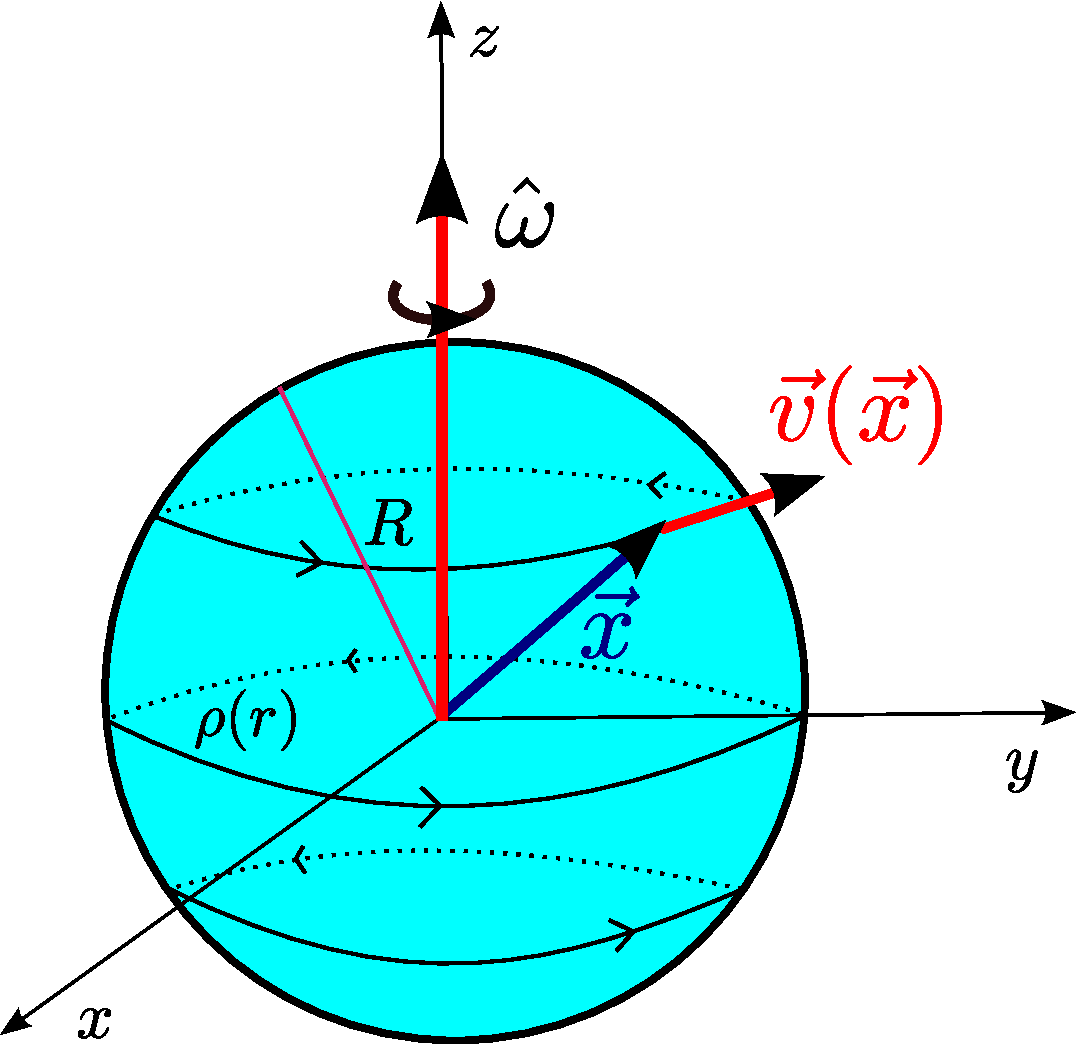
\includegraphics[angle=0,width=0.4\textwidth]{fig/fig-fuente.pdf}
\caption{Modelo de fuente de campo gravitacional: Una distribución de masa esféricamente simétrica que rota, uniforme- y lentamente, en torno a un eje fijo.}
\label{fig:fuente}
\end{figure}

El campo de velocidades $\vec{v}(\vec{x})$ es entonces
\begin{align}
\vec{v}(\vec{x})={}&\vec{\omega}(r)\times\vec{x},
\end{align}
donde $\vec{\omega}=\omega(r)\hat{\omega}$ es la velocidad angular de la distribución con respecto a la dirección fija $\hat{\omega}$. Suponemos que la rapidez angular $\omega(r)$ sólo depende de la distancia radial $r$. El vector $\vec{x}$ puede ser escrito como
\begin{equation}
\vec{x}=r\, \hat{r}=r\left(\hat{\rho}\sin\theta +\hat{z}\cos\theta\right),
\end{equation}
con $\hat{\rho}=\hat{x}\cos\varphi+\hat{y}\sin\varphi$. Además, podemos elegir la orientación del sistema coordenado de modo que el eje de rotación sea el eje $z$, es decir, $\hat{\omega}=\hat{z}$, con lo que $\vec{v}(\vec{x})$ se reduce a
\begin{align}
\vec{v}(\vec{x})={}&\omega(r)r(\hat{z}\times\hat{r})\\
 ={}&\omega(r)r\sin \theta (\hat{z}\times\hat{\rho})\\
 ={}&\omega(r)r\sin \theta\, \hat{\varphi} ,\label{campovelocidad}
\end{align}
donde $\hat{\varphi }=\hat{z}\times\hat{\rho}=-\hat{x}\sin\varphi +\hat{y}\cos\varphi $.

Ahora que ya tenemos una expresión general para el campo de velocidades de la distribución, calculemos su momentum angular total $\vec{J}$, dado por
\begin{equation}
\vec{J}=\int_V \vec{x}\times(\rho \vec{v})\,d^3x.\label{momentumangular}
\end{equation}
Reemplazando (\ref{campovelocidad}) en (\ref{momentumangular}), podemos escribir
\begin{align}
\vec{J}={}&\int_V \rho (r)\omega(r)\sin \theta r^2(\hat{r}\times\hat{\varphi })d^3x\\
 ={}&\int_0^{2\pi}d\varphi \int_0^{\pi}d\theta \int_0^{R}dr\ \rho (r)\omega(r)\sin^2 \theta r^4\left(\sin \theta \hat{z}-\cos \theta \hat{\rho}\right)\\
 ={}&\hat{z}\int_0^{2\pi}d\varphi \int_0^{\pi}d\theta \sin^3 \theta  \int_0^{R}dr\ \rho (r)\omega(r)r^4\nonumber\\
 {}&-\int_0^{2\pi}d\varphi \ \hat{\rho}\int_0^{\pi}d\theta \sin^2 \theta \cos \theta  \int_0^{R}dr\ \rho (r)\omega(r)r^4.\label{j2}
\end{align}
Si además reemplazamos las integrales $\int_0^{2\pi}\hat{\rho}\,d\varphi =\vec{0}$, $\int_0^{\pi}\sin^3\theta\,d\theta  ={4}/{3}$ en (\ref{j2}), obtenemos
\begin{equation}\boxed{
\vec{J}=\frac{8\pi}{3}\int_0^{R}\rho (r)\vec{\omega}(r)r^4\, dr.}\label{jgeneral}
\end{equation}

Calculemos ahora, a partir de la definición \eqref{defAret}, el potencial gravitomagnético $\vec{A}$ que produce esta distribución de masa:
\begin{align}
\vec{A}(\vec{x})={}&-\frac{4G}{c}\int_V \frac{\rho (r') \vec{v}(\vec{x}')}{|\vec{x}-\vec{x}'|}\ d^3x'\\
 ={}&-\frac{4G}{c}\int_V \frac{\rho (r') \vec{\omega}(r')\times\vec{x}'}{|\vec{x}-\vec{x}'|}\ d^3x'\\
 ={}&-\frac{4G}{c}\int_0^{R}dr'r'^2\rho (r')\vec{\omega}(r')\times\left[\int_{\Omega}\frac{\vec{x}'}{|\vec{x}-\vec{x}'|}\ d\Omega'\right],\label{Aradialangular}
\end{align}
La integral angular en \eqref{Aradialangular} es conocida, y su valor es
\begin{equation}
\int_{\Omega}\frac{\vec{x}'}{|\vec{x}-\vec{x}'|}d\Omega'=
\dfrac{4\pi}{3}\frac{r'^2}{r^3}\, \vec{x}, \qquad r'<r .\label{intangular2}
\end{equation}
Reemplazando (\ref{intangular2}) en (\ref{Aradialangular}), obtenemos
\begin{align}
\vec{A}(\vec{x})={}&-\frac{16\pi G}{3cr^3}\int_0^{R}dr'r'^4\rho (r')\vec{\omega}(r')\times\vec{x}\\
={}&\frac{16\pi G}{3cr^3}\ \vec{x}\times\int_0^{R}dr'r'^4\rho (r')\vec{\omega}(r').\label{Acasi}
\end{align}

La integral en (\ref{Acasi}) es proporcional al momentum angular total $\vec{J}$ de la distribución, dado por \eqref{jgeneral}. De este modo encontramos una expresión para el potencial gravitomagnético $\vec{A}(\vec{x})$ en términos del momentum angular $\vec{J}$:
\begin{equation}\boxed{
\vec{A}(\vec{x})=-\frac{2G}{c}\ \frac{\vec{J}\times\vec{x}}{r^3},\qquad r>R.}\label{Afinal}
\end{equation}
Note que esta expresión tiene la misma forma (salvo factores que involucran las constantes gravitacionales y electromagnéticas) que el potencial vectorial electromagnético producido por un \textit{dipolo magnético} (ideal) con momento dipolar magnético $\vec{\mu}$.

Calculando el rotor de \eqref{Afinal} obtenemos la expresión final para el campo gravitomagnético estacionario, producido por la esfera rotante con momentum angular constante $\vec{J}$:
\begin{equation}\boxed{
\vec{H}(\vec{x})=-\frac{2G}{c}\ \frac{3(\vec{J}\cdot\hat{r})\hat{r}-\vec{J}}{r^3},\qquad r>R.}\label{Hgravito}
\end{equation}

Por otro lado, el potencial gravitoeléctrico estacionario producido por la distribución de masa continua siendo el newtoniano, es decir,
\begin{equation}\boxed{
\phi(\vec{x})=-\frac{GM}{r},\qquad r>R,}\label{phifinal}
\end{equation}
donde $M$ es la masa total de la distribución definida como es usual por,
\begin{equation}
M:=\int_V \rho (\vec{x})\, d^3x,\label{masatotal}
\end{equation}

Finalmente, el campo gravitoeléctrico, de acuerdo a \eqref{cge}, es
\begin{equation}\boxed{
\vec{g}(\vec{x})=-\frac{GM}{r^2}\hat{r},\qquad r>R.}\label{ggravito}
\end{equation}

Pensando en la analogía con la electrodinámica, este resultado es idéntico en forma al campo electroestático producido por una distribución de carga esféricamente simétrica con carga total $Q$.

En la figura \ref{fig:gravitoelectromagnetico} podemos ver un esquema de las líneas de campo gravitoeléctrico y gravitomagnético que produce la distribución de masa rotante. Esta fuente de campo se caracteriza completamente por su momentum angular total $\vec{J}$ y por su masa total $M$.
\begin{figure}[H]
\centering
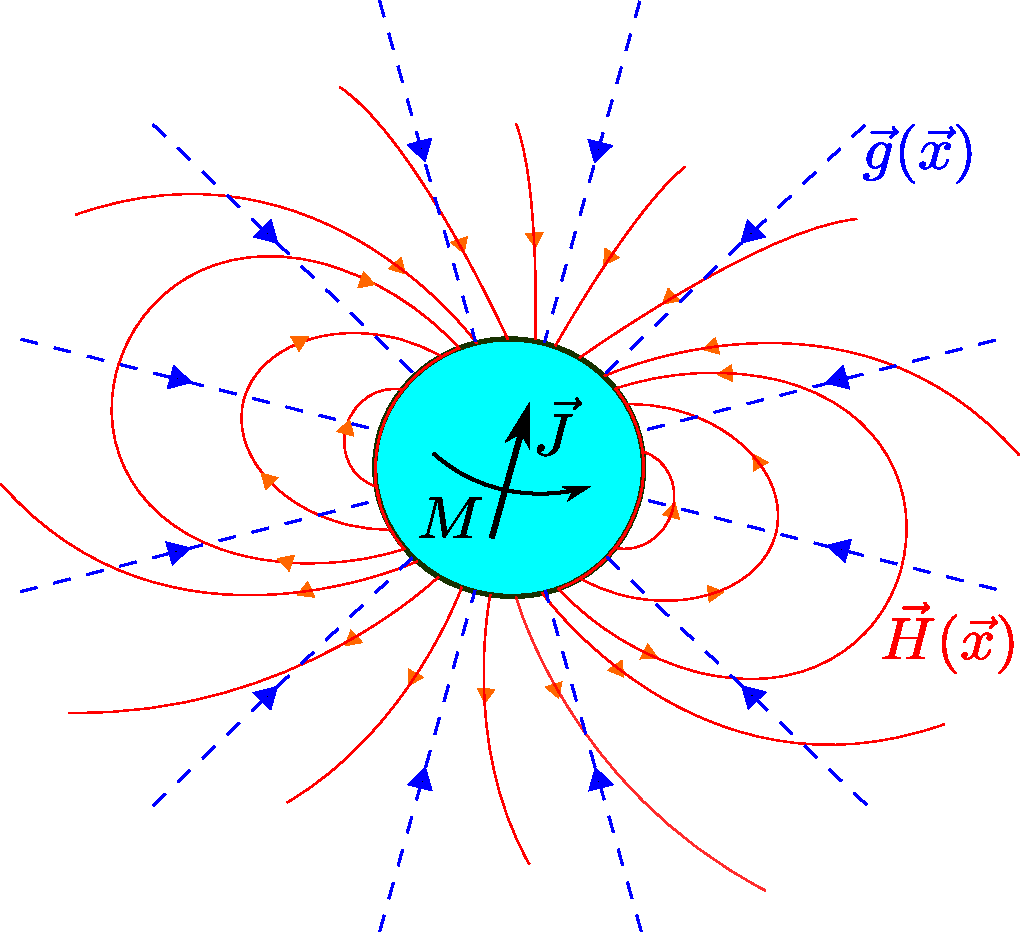
\includegraphics[angle=0,width=0.5\textwidth]{fig/fig-gravitoelectromagnetico.pdf}
\caption{Líneas de campo gravitoeléctrico y gravitomagnético, producidas por una distribución esféricamente simétrica de masa total $M$ y que rota con momentum angular total constante $\vec{J}$.}
\label{fig:gravitoelectromagnetico}
\end{figure}

Note que las líneas de campo gravitomagnético mostradas en \ref{fig:gravitoelectromagnetico} tienen sentido opuesto al del campo magnético generado por una distribución rotante de carga (positiva). Esto se suma al conocido hecho que las líneas de campo gravitoeléctrico tienen sentido opuesto a las del campo eléctrico producido por cargas positivas.

Para finalizar el análisis de esta sección, comparemos los órdenes de magnitud de los campos $\vec{g}$ y $\vec{H}$, producidos por la esfera rotante. De las expresiones (\ref{Hgravito}) y (\ref{ggravito}), podemos ver que estos campos son del orden,
\begin{equation}\label{magg}
g\sim \frac{GM}{R^2}, \qquad H\sim \frac{GJ}{cR^3}.
\end{equation}
Para estimar el orden de magnitud de $J$ podemos hacer $J\sim I\omega\sim MvR$, con lo que obtenemos
\begin{equation}
\frac{H}{g}\sim\frac{v}{c}\ll 1.
\end{equation}

Vemos que, debido a las velocidades no-relativistas de la fuente, el campo gravitomagnético producido es mucho menor en magnitud el correspondiente campo gravitoeléctrico. Por ejemplo, para el Sol y la Tierra $v/c\sim10^{-6}$, por lo que en estos casos $\vec{H}$ es al menos seis órdenes de magnitud menor que $\vec{g}$.

\subsection{Geometría del espaciotiempo fuera de la distribución de masa esférica rotante}

Retornando a la descripción geométrica de la teoría, podemos determinar la métrica  y el elemento de línea del espaciotiempo fuera de la distribución esférica rotante, en términos de los parámetros que caracterizan a la fuente: su masa total $M$ y su momentum angular total $\vec{J}$.

El eje fijo de rotación de la distribución rompe la simetría esférica que tendría el espaciotiempo si la fuente estuviese estática. Sin embargo, persiste una simetría axial remanente  en torno a la dirección definida por el eje de rotación del cuerpo. Sin pérdida de generalidad, podemos elegir un sistema coordenado en que el eje de rotación del cuerpo coincida con el eje $z$, de tal forma que el momentum angular de la distribución se pueda expresar en la forma,
\begin{equation}
\vec{J}=J\hat{z}.
\end{equation}
En este caso, se tiene que los potenciales $\phi$ y $\vec{A}$ toman una forma más simple,
\begin{equation}
\phi(r) = -\frac{GM}{r},\label{phiii}\\
\end{equation}
\begin{equation}
\vec{A}(r,\theta,\varphi ) = -\frac{2GJ}{c}\frac{\hat{z}\times\hat{r}}{r^2}
=-\frac{2GJ}{c}\frac{\sin \theta }{r^2}\hat{\varphi}%=-\frac{2GJ}{c}\frac{\sin \theta }{r^2}\left[-\hat{x}\sin\varphi +\hat{y}\cos\varphi\right]
.\label{aphii}
\end{equation}
Si reemplazamos ahora \eqref{aphii} en \eqref{ds2phiA}, obtenemos el elemento de línea:
%\begin{equation}
%g_{\mu\nu}(x):=
%\left( \begin{array}{cccc}
%\vspace{4mm}
%1-\frac{2GM}{c^2r} & -\frac{2GJ}{c^3r^2}\sin \theta \sin\varphi & \frac{2GJ}{c^3r^2}\sin \theta \cos\varphi & 0 \\
%\vspace{4mm}
%-\frac{2GJ}{c^3r^2}\sin \theta \sin\varphi &-1-\frac{2GM}{c^2r} & 0 & 0 \\
%\vspace{4mm}
%\frac{2GJ}{c^3r^2}\sin \theta \cos\varphi & 0 &-1-\frac{2GM}{c^2r} & 0 \\
%0 & 0 & 0 &-1-\frac{2GM}{c^2r} \\
%\end{array} \right)+\mathcal{O}(G^2).\label{grafica2}
%\end{equation}
\begin{equation}
ds^2=\left(1-\frac{2GM}{c^2r}\right)c^2dt^2-\left(1+\frac{2GM}{c^2r}\right)d\vec{x}^2+\frac{4GJ}{c^3r^2}\sin\theta (\hat\varphi\cdot d\vec{x})cdt+\mathcal{O}(G^2).\label{ds22}
\end{equation}
En coodenadas esféricas, sabemos que $\hat\varphi\cdot d\vec{x}=r\sin\theta\,d\varphi$, y por lo tanto la expresión a primer orden en $G$ para el elemento de línea fuera de la distribución esférica rotante, en coordenadas esféricas y en términos de $M$ y $J$, resulta ser
\begin{equation}\boxed{
ds^2=\left(1-\frac{2GM}{c^2r}\right)c^2dt^2-\left(1+\frac{2GM}{c^2r}\right)\left[dr^2+r^2d\Omega^2\right]+\frac{4GJ}{c^3r}\sin^2 \theta d\varphi (cdt)+\mathcal{O}(G^2).}\label{dssss2}
\end{equation}
Es posible verificar que la solución exacta del agujero negro rotante de Kerr en coordenadas isotrópicas, se reduce a (\ref{dssss2}) en el límite de campo debil. Si adicionalmente hacemos $J=0$ recobramos la solución de Schwarzschild, a primer orden en $G$, también en coordenadas isotrópicas.

\section{Estudio de órbitas y resolución perturbativa de la ecuación del movimiento para una partícula ligada y no-relativista en el espaciotiempo fuera de una esfera rotante.}

\section{Precesión Relativista de Giróscopos}

Una de las formas de testear las predicciones de RG respecto al campo gravitomagnético, es describiendo los efectos que la presencia de éste campo produce sobre \textit{pequeños cuerpos de prueba con movimiento interno de rotación} (``spin"), es decir, sobre lo que llamaremos un \textit{giróscopo}.

\subsection{Giróscopos y 4-vector de spin}

Modelamos un giróscopo como un pequeño cuerpo caracterizado no sólo por %su masa $m$, 
su posición $\vec{x}(t)$ y su velocidad $\vec{v}(t)$, sino que además por un \textit{vector de momentum angular de rotación propia} o \textit{spin} $\vec{S}(t)$, que describe la rotación en torno a su propio eje. En la práctica se construyen giróscopos mecánicos y ópticos (ver \cite{1} para más detalles.)
%El momentum lineal del cuerpo se define como es usual:
%\begin{align}
%\vec{p}:=m\vec{v}
%\end{align}
%y su momentum angular orbital por
%\begin{align}
%\vec{L}:=\vec{x}\times\vec{p}.
%\end{align}

La propiedad básica de un giróscopo, es que \textit{en ausencia de fuerzas y torques externos ellos mantienen constante la magnitud y dirección de su spin $\vec{S}$}, respecto a un SRI, es decir, 
\begin{align}
\frac{d\vec{S}}{dt}=\vec{0}.\label{dinamicaS1}
\end{align}


Como sabemos, para describir el movimiento de un cuerpo en la Teoría Especial de la Relatividad, es útil parametrizar las cantidades usando el tiempo propio $\tau$ y definir la 4-posición del objeto $x^\mu (\tau)$, además de su 4-velocidad $u^\mu (\tau)$. Por otro lado, para describir el vector de spin $\vec{S}$, definimos un \textit{4-vector de spin} $S^\mu (\tau)$, tal que en el SRI comóvil con el giróscopo sólo tiene componentes espaciales:
\begin{align}
S^\mu \stackrel{*}{=}(0,\vec{S}).
\end{align}
Puesto que en este SRI la 4-velocidad del cuerpo es dada por $u^\mu\stackrel{*}{=}(u^0,\vec{0})$, entonces se tiene $S^\mu u_\mu\stackrel{*}{=}0$. Como consecuencia $S^{\mu}$ es ortogonal a $u^{\mu}$ en todo SRI, ya que $S^\mu u_\mu$ es un escalar:
\begin{equation}\boxed{\label{escalarSu2}
S^\mu u_\mu=0.}
\end{equation}

Además, como la 4-velocidad del giróscopo es un 4-vector tipo tiempo, es decir $u^{\mu}u_{\mu}>0$, entonces de (\ref{escalarSu2}) se desprende que $S^{\mu}$ es siempre un vector tipo espacio, es decir, $S^\mu S_{\mu}<0$.

Así, en Relatividad Especial, un giróscopo será descrito por 
%su masa $m$, 
su 4-posición $x^{\mu}(\tau)$, su 4-velocidad $u^{\mu}(\tau)$ y su vector de spin $S^{\mu}(\tau)$, tal como se ilustra en la figura \ref{giroscopo}. La ecuación que describe la dinámica de $S^{\mu}$, en ausencia de fuerzas y torques externos, se debe reducir a (\ref{dinamicaS1}), y es dada en cualquier SRI por
\begin{equation}\boxed{
\frac{dS^{\mu}}{d\tau}=0.}\label{dinamicaS2}
\end{equation}
\begin{figure}[H]
\centering
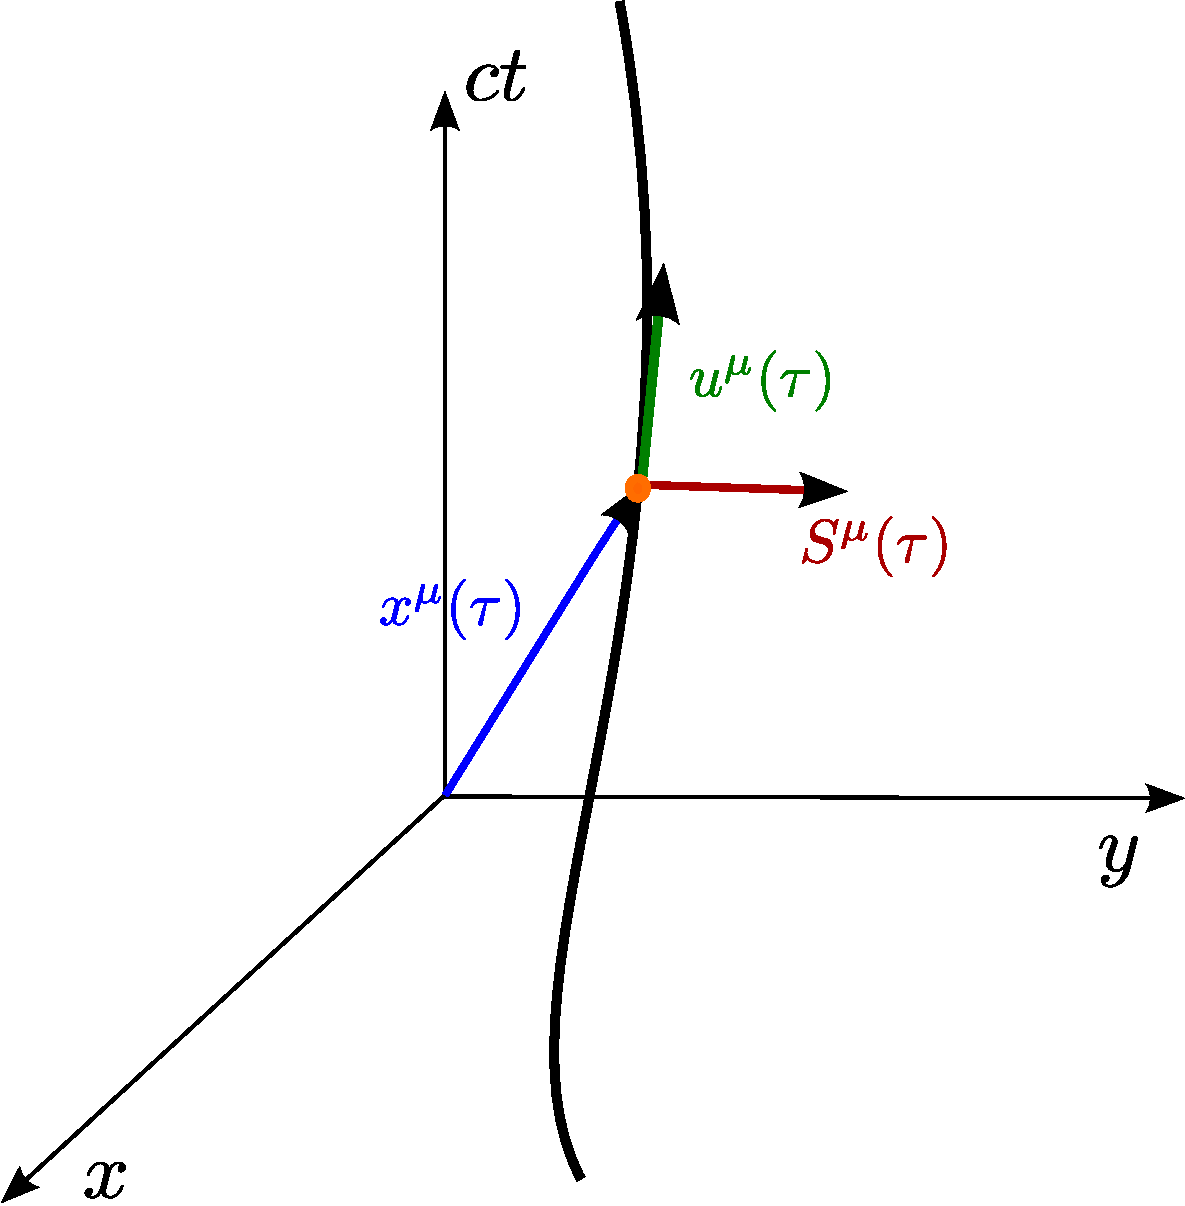
\includegraphics[angle=0,width=0.4\textwidth]{fig/fig-giroscopo.pdf}
\caption{Un giróscopo.}
\label{giroscopo}
\end{figure}

\subsection{Determinación de la velocidad angular de precesión del spin de un giróscopo moviéndose en una geodésica bajo la acción del campo gravitomagnético.}

Consideremos un giróscopo que se mueve en el espaciotiempo fuera de una fuente de campo gravitacional, con 4-velocidad
\begin{equation}
u^\mu (\tau):=\frac{dx^\mu }{d\tau}.
\end{equation}
Requerimos una ecuación de evolución para el vector $S^\mu$ en un campo gravitacional no nulo. Para encontrarla, hacemos uso del principio de equivalencia de Einstein. En ausencia de gravitación (y además de fuerzas y torques netos de otras fuerzas), la dirección y magnitud del vector de spin es constante respecto a un SRI. Por lo tanto, lo mismo debe ocurrir, de acuerdo a este principio, en un SRLI. Si $\bar{x}^\mu$ son las coordenadas geodésicas asociadas a un SRLI, entonces (ver \eqref{dinamicaS2}): 
\begin{equation}\label{dSdtauast0}
\frac{d\bar{S}^\mu }{d\tau}\stackrel{*}{=}0.
\end{equation}
En coordenadas arbitrarias, tendremos
\begin{equation}\label{fwt}
\boxed{\frac{DS^\mu }{D\tau}=0,}
\end{equation}
donde hemos introducido la \textit{derivada covariante a lo largo de la línea de mundo $x^\mu(\tau)$}:
\begin{equation}\label{DSDtau}
\frac{DS^\mu}{D\tau}:=\frac{dS^\mu}{d\tau}+\Gamma^{\mu}_{\ \nu\lambda}S^\nu u^\lambda .
\end{equation}
Claramente, la ecuación \eqref{fwt} se reduce a \eqref{dSdtauast0} en coordenadas geodésicas, ya que las componentes de la conexión se anulan\footnote{Note que este resultado es válido para \textit{todo evento sobre la línea de mundo} $x^\mu(\tau)$.}. Además, \eqref{DSDtau} es un vector bajo TGC's. Esto puede verificarse fácilmente notando que podemos escribir
\begin{equation}
\frac{DS^\mu}{D\tau}:=u^\nu\nabla_\nu S^\mu,
\end{equation}
que es la generalización covariante de la derivada respecto al tiempo propio $\tau$ (que mide un observador comóvil con el giróscopo) a lo largo de la trayectoria $x^\mu (\tau)$:
\begin{equation}
\frac{dS^\mu }{d\tau}=u^{\nu}\partial_{\nu} S^{\mu}.
\end{equation}
%Cualquier 4-vector que satisfaga una ecuación de la forma de (\ref{fwt}), se dice que efectúa un transporte de ``Fermi-Walker'' a lo largo de su trayectoria.

Si contraemos la ecuación (\ref{fwt}) con $S_{\mu}$, completamos la derivada covariante total, parametrizada con respecto a $\tau$, y usamos el hecho que para un escalar la derivada covariante coincide con la derivada parcial, se encuentra que $S^\mu S_{\mu}$ es una \textit{constante del movimiento}, es decir,
\begin{equation}\boxed{
\frac{d\ }{d\tau}\left(S^\mu S_{\mu}\right)=0.}\label{SSconstante}
\end{equation}

En particular, consideremos el caso de un giróscopo que orbita (dentro de un satélite) una fuente de campo gravitacional (la Tierra, por ejemplo). Supongamos que el satélite está construido de tal forma que es capaz de proteger al giróscopo de toda influencia externa no-gravitacional, haciendo que su 4-aceleración $a^\mu $ sea nula y por consiguiente el giróscopo se mueva en una geodésica bajo la acción del campo gravitacional,
\begin{equation}
a^\mu (\tau):=\frac{d^2x^\mu }{d\tau^2}+\Gamma^\mu _{\ \nu\lambda}\frac{dx^{\nu}}{d\tau}\frac{dx^{\lambda}}{d\tau}=0.
\end{equation}
Bajo estas consideraciones,  las ecuaciones (\ref{fwt}) y (\ref{SSconstante}) son válidas para describir la dinámica del 4-vector de spin $S^{\mu}(\tau)$.

En la figura \ref{GPB} se muestra gráficamente el problema que queremos analizar para el caso particular de un giróscopo dentro de un satélite que orbita la Tierra, como es el caso del proyecto GPB.
\begin{figure}[H]
\centering
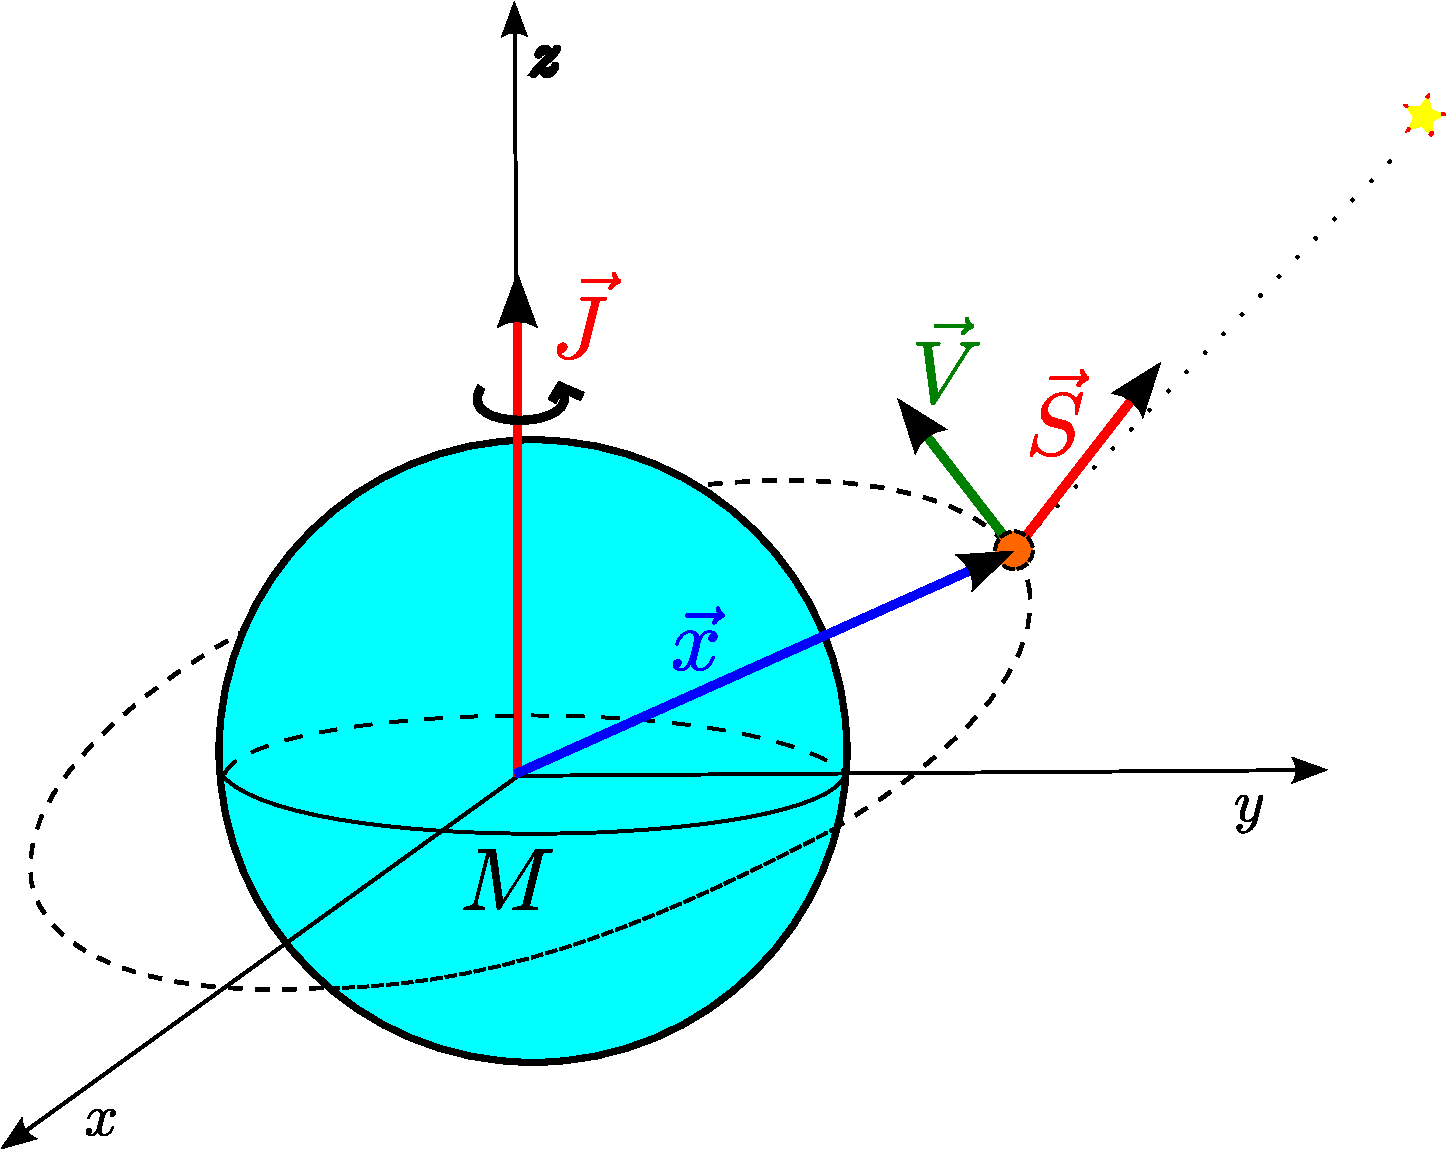
\includegraphics[angle=0,width=0.5\textwidth]{fig/fig-GPB.pdf}
\caption{Giróscopo que describe una geodésica en torno a la Tierra.}
\label{GPB}
\end{figure}
Ahora expresamos las derivadas en \eqref{escalarSu2}, \eqref{fwt} con \eqref{DSDtau} y  \eqref{SSconstante} en términos de la coordenada temporal $t$ del observador cuasi-inercial, con lo que obtenemos 
\begin{align}
\frac{dS^\mu }{dt}+\Gamma^\mu _{\ \nu\lambda}S^{\nu}\frac{dx^{\lambda}}{dt}={}&0,\label{giro1}\\
g_{\mu\nu}S^\mu S^{\nu}={}&\text{cte},\label{giro2}\\
g_{\mu\nu}S^\mu \frac{dx^{\nu}}{dt}={}&0.\label{giro3}
\end{align}
El paso siguiente es calcular las ecuaciones \eqref{giro1}-\eqref{giro3}, consistentemente hasta orden $G^{3/2}$, reescribiéndolas en términos de la velocidad $v^i=dx^i/dt$ del giróscopo, el vector de spin $S^i$ (componentes espaciales) y los potenciales $\phi$ y $A^i$.

Primero, si evaluamos (\ref{giro1}) para $\mu=i$ y notamos que $dx^{0}/dt=c$, encontramos
\begin{equation}
\frac{dS^{i}}{dt}+c\Gamma^{i}_{\ 00}S^{0}+\Gamma^{i}_{\ 0j}S^{0}v^j+c\Gamma^{i}_{\ j0}S^{j}+\Gamma^{i}_{\ jk}S^{j}v^k=0.\label{giro12}
\end{equation}
Luego, si reemplazamos en (\ref{giro12}), los valores de los símbolos de Christoffel dados en (\ref{simbolo1})-(\ref{simbolo6}), obtenemos
\begin{align}
\frac{dS^{i}}{dt}={}&-\frac{1}{c}(\partial_i\phi)S^0+\frac{1}{2c^2}(\partial_i A^j-\partial_j A^i)S^0v^j+\frac{1}{c^3}\frac{\partial \phi}{\partial t}S^0v^i+\frac{1}{2c}(\partial_i A^j-\partial_j A^i)S^j+\frac{1}{c^2}\frac{\partial \phi}{\partial t}S^i\nonumber\\
{}&-\frac{1}{c^2}(\partial_i \phi) S^jv^j+\frac{1}{c^2}v^j(\partial_j\phi)S^i+\frac{1}{c^2}(\partial_j \phi) S^jv^i+\mathcal{O}(G^2)\label{dsidt}.
\end{align}

%Por otra parte, usando las expresiones para las componentes de la métrica $g_{\mu\nu}$ en términos de los potenciales, dadas en (\ref{gphiA}), podemos escribir explícitamente (\ref{giro2}) hasta orden $G$:
%\begin{equation}
%(S^0)^2+\frac{2}{c^2}\phi(S^0)^2-\frac{2}{c^2}A^iS^0S^i-S^iS^i+\frac{2}{c^2}\phi S^iS^i+\mathcal{O}(G^2)=\text{cte}.\label{sisicte}
%\end{equation}
Necesitamos escribir $S^0$ en términos de las demás cantidades, para lo cual la ecuación (\ref{giro3}) nos será útil:
\begin{align}
S^0+\frac{2\phi}{c^2}S^0-\frac{1}{c^3}A^iv^iS^0-\frac{1}{c^2}A^iS^i-\frac{1}{c}S^iv^i 
+\frac{2\phi}{c^3}S^iv^i+\mathcal{O}(G^2)=0.\label{giro32}
\end{align}
Podemos despejar $S^0$ de \eqref{giro32}. Notamos sin embargo, que para ser reemplazada en \eqref{dsidt} sólo requerimos conocer $S^0$ a orden 0 en potencias de $G$ (ya que siempre aparece multiplicada por términos de orden 1). Por lo tanto, nos basta con escribir:
\begin{equation}
S^0=\frac{1}{c}v^iS^i +\mathcal{O}(G).\label{S00}
\end{equation}
%Note que el término $(S^iv^i)(A^jv^j)/c^4$ ha sido despreciado debido a que es de orden $G^2$, pues $v^i\sim G^{1/2}$. 
%A partir de \eqref{S00} calculamos $(S^0)^2$ quedándonos con términos hasta orden $G^{3/2}$:
%\begin{equation}
%(S^0)^2=\frac{1}{c^2}(v^iS^i)(v^jS^j)+\frac{2}{c^3}(A^iS^i)(v^jS^j)+\mathcal{O}(G^2).\label{S002}
%\end{equation}
Finalmente, si reemplazamos \eqref{S00} %y \eqref{S002} 
en \eqref{dsidt}, y suponemos que el campo gravitacional es estacionario, 
obtenemos dos ecuaciones en que sólo aparecen $S^i$, $v^i$, $\phi$ y $A^i$, dadas por
\begin{align}
\frac{dS^{i}}{dt} &= \frac{1}{2c}\left(\partial_iA^j-\partial_jA^i\right)S^j + \frac{1}{2c^3}(\partial_iA^j-\partial_jA^i)v^jv^kS^k \nonumber \\
&\quad  -\frac{2}{c^2}(\partial_i\phi) S^jv^j+\frac{1}{c^2}(\partial_j\phi)v^jS^i+\frac{1}{c^2}(\partial_j\phi)S^jv^i+\mathcal{O}(G^2).\label{dsidt2}
\end{align}
%\begin{equation}
%S^iS^i-\frac{2\phi}{c^2}S^iS^i-\frac{1}{c^2}(v^iS^i)^2+\mathcal{O}(G^2)=\text{cte}.\label{sisicte2}
%\end{equation}
%La ecuación (\ref{sisicte2}) sugiere definir el vector de spin auxiliar 
%\begin{equation}\boxed{
%{\cal L}^i:=\left(1-\frac{1}{c^2}\phi\right)S^i-\frac{1}{2c^2}v^i(v^jS^j),}\label{defli}
%\end{equation}
%cuyo módulo cuadrado reproduce precisamente el lado izquierdo de \eqref{sisicte2}, y por lo tanto satisface 
%\begin{equation}
%{\cal L}^i{\cal L}^i=\text{cte.}+\mathcal{O}(G^2) ,\label{lilicte}
%\end{equation}
%es decir, que su módulo cuadrado es constante a orden $G^{3/2}$.
%
%Expresamos ahora la ecuación \eqref{dsidt2} en términos de la variable auxiliar ${\cal L}^i$. Para ello, calculamos su derivada temporal a partir de su definición en \eqref{defli}:
%\begin{equation}
%\frac{d{\cal L}^i}{dt}=-\frac{1}{c^2}\frac{\partial\phi}{\partial t}S^i-\frac{1}{c^2}v^j(\partial_j\phi)S^i+\frac{dS^i}{dt}-\frac{\phi}{c^2}\frac{dS^i}{dt}-\frac{1}{2c^2}v^jS^j\frac{dv^i}{dt}-\frac{1}{2c^2}v^iS^j\frac{dv^j}{dt}-\frac{1}{2c^2}v^iv^j\frac{dS^j}{dt}.\label{dlidt}
%\end{equation}
%Luego, reemplazando (\ref{dsidt2}) y la ecuación del movimiento (\ref{movnorel}) en (\ref{dlidt}), se obtiene la siguiente ecuación que incluye términos hasta  orden $G^{3/2}$:
%\begin{align}
%\frac{d{\cal L}^i}{dt}=\frac{1}{2c}(\partial_iA^j-\partial_jA^i)S^j+\frac{3}{2c^2}\left(v^i\partial_j\phi-v^j\partial_i\phi\right)S^j+\mathcal{O}(G^2).\label{dlidt2}
%\end{align}
%Finalmente, podemos reemplazar $S^j$ por ${\cal L}^j$ en el lado derecho de (\ref{dlidt2}), ya que ambas cantidades difieren en términos de orden mayor o igual a $G$. Además, si utilizamos el símbolo de Levi-Civita, obtenemos
%\begin{equation}
%\frac{d{\cal L}^i}{dt}=\frac{1}{2c}\epsilon_{ijk}{\cal L}^j\left(\epsilon_{klm}\partial_l A^m\right)+\frac{3}{2c^2}\epsilon_{ijk}{\cal L}^k\left(\epsilon_{jlm}v^l\partial_m\phi\right)+\mathcal{O}(G^2),\label{dlidt3}
%\end{equation}
%y en notación vectorial,
%\begin{equation}\boxed{
%\frac{d\vec{{\cal L}}}{dt}=\left[-\frac{1}{2c}(\vec{\nabla}\times\vec{A})-\frac{3}{2c^2}(\vec{v}\times\vec{\nabla}\phi)\right]\times\vec{{\cal L}}+\mathcal{O}(G^2).}
%\end{equation}
esta ecuación puede reescribirse como 
\begin{align}
\frac{dS^i}{dt} =& \frac{1}{2c}\epsilon_{ijk}S^j\left(\epsilon_{klm}\partial_l A^m\right)+\frac{3}{2c^2}\epsilon_{ikj}S^k\left(\epsilon_{jlm}v^l\partial_m\phi\right)
+ \frac{1}{2c^3}\epsilon_{ijk}v^j(\epsilon_{klm}\partial_l A^m)v^p S^p\nonumber\\
& +\frac{1}{2c^2}\left[2(\partial_j\phi)v^jS^i-(\partial_i\phi)v^jS^j -(\partial_j\phi)v^iS^j\right]+\mathcal{O}(G^2),\label{dlidt3}
\end{align}
y en notación vectorial,
\begin{align}\label{dSdtvec}
\frac{d\vec{S}}{dt} &= \left[-\frac{1}{2c}(\vec{\nabla}\times\vec{A})-\frac{3}{2c^2}(\vec{v}\times\vec{\nabla}\phi)\right]\times\vec{S} \nonumber \\
 &\quad +\frac{1}{2c^2}\left[2\vec{S}(\vec{v}\cdot\vec{\nabla}\phi)-(\vec{\nabla}\phi)\vec{v}\cdot\vec{S}-(\vec{S}\cdot\vec\nabla\phi)\vec{v}\right] \nonumber\\
 &\quad + \frac{1}{2c^3}[\vec{v}\times(\vec{\nabla}\times\vec{A})](\vec{v}\cdot\vec{S})+\mathcal{O}(G^2).
\end{align}
En el caso en que la órbita del giróscopo sea ligada, $v\sim G^{1/2}$, y el término en la tercera línea de \eqref{dSdtvec} es de orden $\mathcal{O}(G^2)$, de modo que debe ser despreciado. Así obtenemos
\begin{align}\label{dSdtvecfinal}
\frac{d\vec{S}}{dt} &= \left[-\frac{1}{2c}(\vec{\nabla}\times\vec{A})-\frac{3}{2c^2}(\vec{v}\times\vec{\nabla}\phi)\right]\times\vec{S} \nonumber \\
 &\quad +\frac{1}{2c^2}\left[2\vec{S}(\vec{v}\cdot\vec{\nabla}\phi)-(\vec{\nabla}\phi)\vec{v}\cdot\vec{S}-(\vec{S}\cdot\vec\nabla\phi)\vec{v}\right] +\mathcal{O}(G^2).
\end{align}
Escribimos esta expresión como
\begin{equation}
\frac{d\vec{S}}{dt}=\vec{\Omega}\times\vec{S}+\cdots + \mathcal{O}(G^2),
\end{equation}
donde hemos definido,
\begin{equation}
\vec{\Omega}:=\vec{\Omega}_{\rm GEO}+\vec{\Omega}_{\rm LT},
\end{equation}
con $\vec{\Omega}_{\rm GEO}$ la velocidad angular de precesión \emph{geodésica}, dada por
\begin{align}\boxed{
\vec{\Omega}_{\rm GEO}:=\frac{3}{2c^2}(\vec{v}\times\vec{g}),}\label{geodetic}
\end{align}
y $\vec{\Omega}_{\rm LT}$ la velocidad angular de precesión de \emph{Lense-Thirring}, 
\begin{align}\boxed{
\vec{\Omega}_{\rm LT}:=-\frac{1}{2c}\vec{H},}\label{LT}
\end{align}
en honor a los dos científicos que en 1918 predijeron este efecto conocido como ``frame-dragging''.


\subsection{Predicción para un giróscopo que orbita la Tierra y que intenta medir el GPB}

Evaluemos las expresiones (\ref{geodetic}) y (\ref{LT}) para el caso de un giróscopo que orbita la Tierra, con lo que podremos obtener la famosa predicción que recientemente midió con éxito el GPB \cite{Everitt11}. Usaremos los campos gravitoeléctro y gravitomagnético, de una masa esféricamente simétrica rotando respecto a un eje fijo, calculados en (\ref{Hgravito}) y (\ref{ggravito}), de modo que en este caso
\begin{align}
\vec{g}(r)={}&-\frac{GM_T}{r^2}\hat{r},\label{gGPB}\\
\vec{H}(r)={}&-\frac{2GJ_T}{cr^3}\left[3(\hat{J}_T\cdot\hat{r})\hat{r}-\hat{J}_T\right]\label{BGPB},
\end{align}
donde $M_T$ es la masa total de la Tierra, $J_T$ su momento angular total y $\hat{J}_T$ el vector unitario la dirección de rotación.

Por simplicidad, supongamos que el giróscopo gira en una \textit{órbita circular} en torno a la Tierra, por lo que su velocidad se puede escribir en forma compacta por
\begin{equation}
\vec{v}=\left(\frac{M_TG}{R}\right)^{1/2}\hat{h}\times\hat{r},\label{aproxcirculo}
\end{equation}
donde $R$ es el radio de la órbita y $\hat{h}$ su vector unitario normal\footnote{Esta órbita circular es una geodésica a primer orden en $G$. Ver por ejemplo \eqref{solucasi}.}. Ver la figura \ref{orbitaGPB}. Luego, reemplazando (\ref{gGPB}), (\ref{BGPB}) y (\ref{aproxcirculo}) en (\ref{geodetic}) y (\ref{LT}), obtenemos
\begin{align}
\vec{\Omega}_{\rm GEO}={}&\frac{3}{2c^2}\frac{M_T^{3/2}G^{3/2}}{R^{5/2}}\left[\hat{h}-(\hat{h}\cdot\hat{r})\hat{r}\right],\label{geo11}\\
\vec{\Omega}_{\rm LT}={}&\frac{GJ_T}{c^2R^3}\left[3(\hat{J}_T\cdot\hat{r})\hat{r}-\hat{J}_T\right].\label{LT11}
\end{align}
Consideremos además el caso particular en que el giróscopo se mueve \textit{en una órbita polar alrededor de la Tierra}, es decir, tal que
\begin{align}
\hat{h}\cdot\hat{J}_T=0,
\end{align}
como se muestra en la figura \ref{orbitaGPB}.
\begin{figure}[H]
\centering
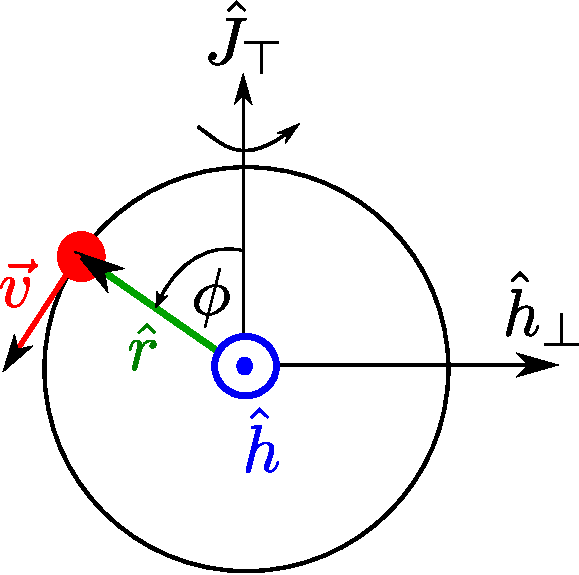
\includegraphics[angle=0,width=0.3\textwidth]{fig/fig-orbitaGPB.pdf}
\caption{Giróscopo en una órbita circular polar en torno a la Tierra.}
\label{orbitaGPB}
\end{figure}
De la figura vemos que podemos parametrizar la órbita por
\begin{align}
\hat{r}(\phi)=\hat{J}_T\cos\phi-\hat{h}_{\perp}\sin\phi,\label{parametrizacionorbita}
\end{align}
donde $\hat{h}_{\perp}$ es un vector unitario perpendicular a $\hat{h}$ y $\hat{J}_T$. Si reemplazamos (\ref{parametrizacionorbita}) en (\ref{geo11}) y (\ref{LT11}), y luego promediamos a lo largo de una órbita completa del giróscopo, es decir, $\phi\in[0,2)$, entonces las \emph{velocidades angulares promedio} de precesión por revolución, quedan dadas finalmente por
\begin{equation}\boxed{
\begin{aligned}
\langle\vec{\Omega}_{\rm GEO}\rangle={}&\frac{3G^{3/2}}{2c^2}\frac{M_T^{3/2}}{R^{5/2}}\hat{h},\\
\langle\vec{\Omega}_{\rm LT}\rangle={}&\frac{G}{2c^2}\frac{J_T}{R^3}\hat{J}_T.\label{LT22}
\end{aligned}}
\end{equation}
Las expresiones (\ref{LT22}) son las predicciones de RG para el caso de un giróscopo orbitando una masa rotante en una órbita circular polar. Para obtener un resultado numérico, consideramos a la Tierra como una esfera de radio $R_T=6.371\times 10^6\,\rm m$ (***diferencia con tabla en apéndice!***) y distribución de masa esféricamente simétrica de masa total $M_T=5.97\cdot 10^{24}\,\rm kg$. Sea la altura de la órbita polar circular de $642\,\rm km$ sobre la superficie de la Tierra, es decir, $h=6.42\times 10^5 \,\rm m$, por lo que se tiene $R=R_T+h=7.013\times 10^{6}\,\rm m$. Para calcular el momentum angular total de rotación de la Tierra, usamos su definición en (\ref{jgeneral}), con lo que obtenemos
\begin{align}
J_T=\frac{2}{5}M_TR_T^2\omega,
\end{align}
y finalmente considerando que el periodo de rotación de la Tierra es $T=23.9345\,\rm hr$, se tiene $\omega=2\pi/T=7.2919\times 10^{-5}\,\rm rad/s$ y por consiguiente $J_T=7.0679\times 10^{33}\,\rm kg\,m^2/s$.
Luego, evaluando todos los datos en (\ref{LT22}), y considerando $G=6.67\times 10^{-11}\,\rm N\,m^2/kg^2$, las predicciones numéricas de RG para la precesión del giróscopo que confirmó el satélite GPB son:
\begin{align}
\langle\vec{\Omega}_{\rm GEO}\rangle={}&6.6{\rm \frac{sec}{yr}}\hat{h},\\
\langle\vec{\Omega}_{\rm LT}\rangle={}&0.049{\rm \frac{sec}{yr}}\hat{J}_T.
\end{align}

***No sé por qué la precesión de Lense-Thirring difiere en $0.005\,\rm sec/yr$ con respecto al resultado de la figura 7.6 y en $0.007\,\rm sec/yr$ con respecto al paper oficial del GPB, que es $\langle\Omega_{\rm LT}\rangle=0.039\,\rm sec/yr$. El resultado experimental medido por GPB fue $\langle\Omega_{\rm LT}{}\rangle_{\rm\bf exp}=(0.0372\pm 0.0072)\,\rm sec/yr$. Para más detalles ver \cite{Everitt11}. ***

\begin{figure}[H]
\centering
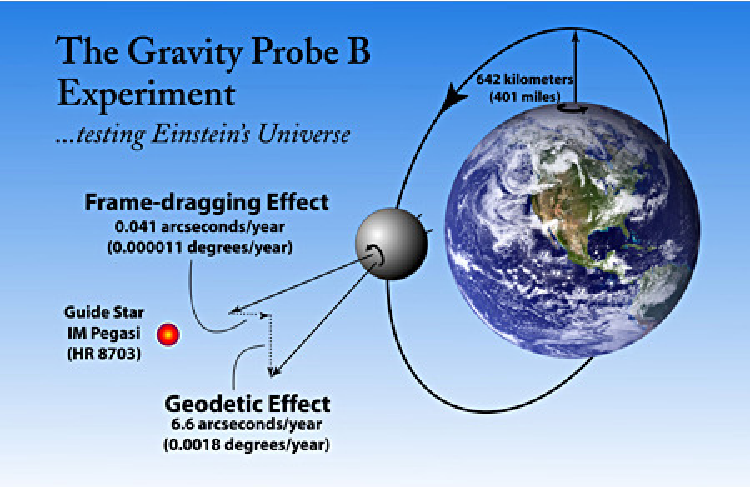
\includegraphics[angle=0,width=0.5\textwidth]{fig/fig-precesion.pdf}
\caption{Esquema de los ángulos de precesión del giróscopo, medidos por la sonda GPB.}
\label{precesion}
\end{figure}